\subsubsection{Dashboard - Tasa de crecimiento vs Consumo de energ�a}

En este panel presentaremos informaciones sobre el consumo y clientes de la ANDE por grupo de consumidores y departamento.

\textsc{\begin{figure}[H]
	\centering
	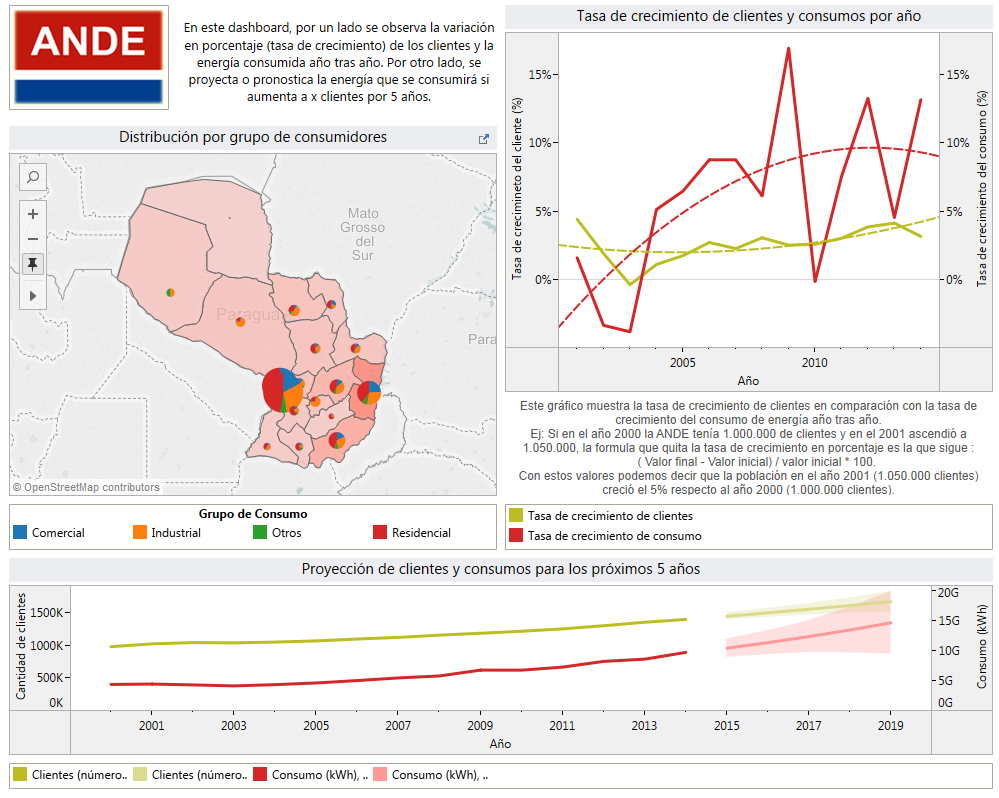
\includegraphics[width=\linewidth]{figuras/TasaDeCrecimientoVsConsumoDeEnergia}
	\caption{Tasa de crecimiento vs Consumo de energ�a}
	\label{fig:TasaDeCrecimientoVsConsumoDeEnergia}
\end{figure}}

En el mapa se presentan gr�ficos de tortas por cada departamento, que representan los grupos de consumidores (Comercial, Industrial, Residencial y otros), donde cada color representa a un grupo en espec�fico. Se puede ver que en la mayor�a de los departamentos el grupo de consumo ``residencial``,  ``industrial`` y ``comercial`` son las que ocupan la mayor porci�n. Estos grupos sirven como filtro para los dem�s gr�ficos, por ejemplo, si se presiona sobre cualquier grupo de consumidores, los dem�s gr�ficos se actualizar�n en tiempo real. Al ubicar el mouse sobre alguna porci�n de la torta, se muestra el consumo equivalente del departamento correspondiente.

\textsc{\begin{figure}[H]
	\centering
	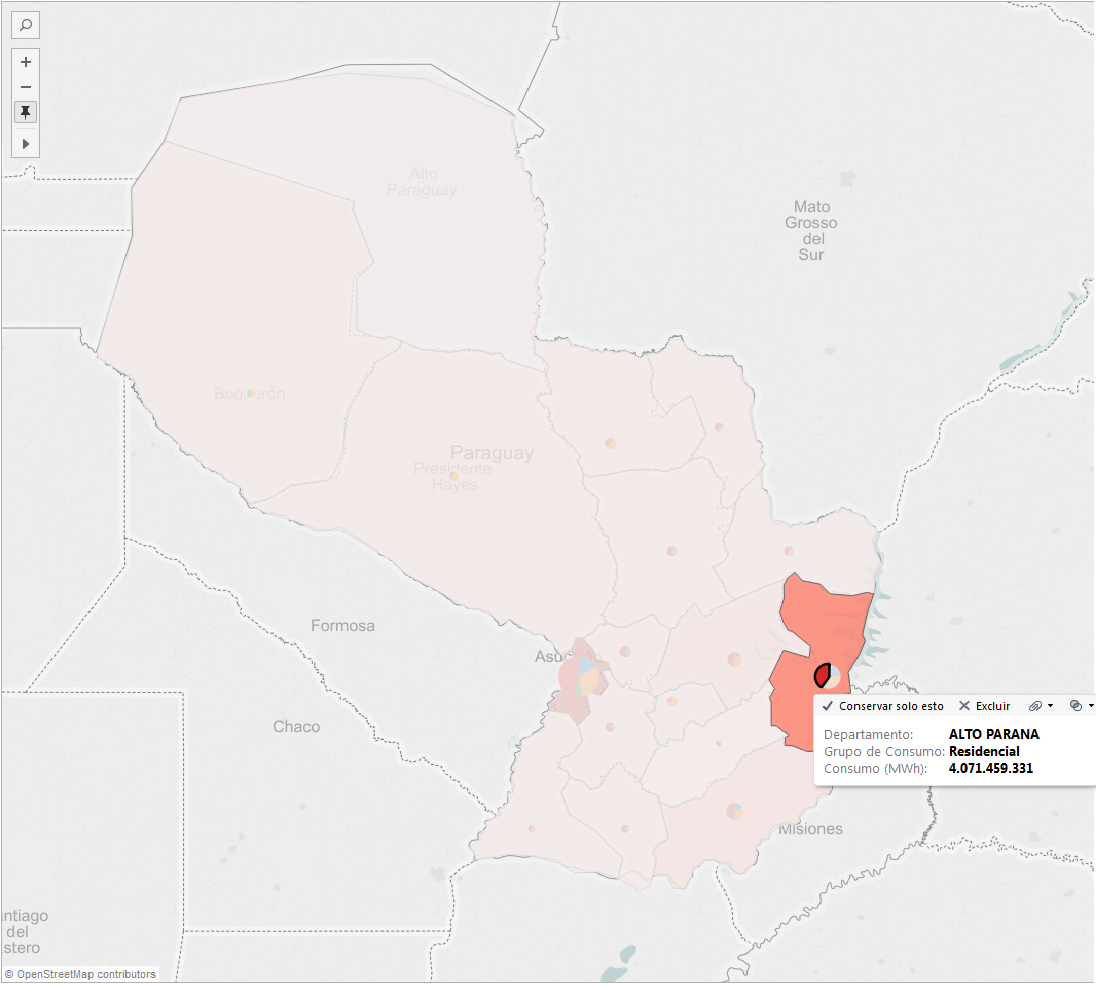
\includegraphics[width=\linewidth]{figuras/TasaDeCrecimientoVsConsumoDeEnergia1}
	\caption{Tasa de crecimiento vs Consumo de energ�a, filtrado por el departamento Alto Paran�}
	\label{fig:TasaDeCrecimientoVsConsumoDeEnergia1}
\end{figure}}


En este gr�fico se utiliz� datos de los clientes de la entidad y el consumo de energ�a el�ctrica.  Se calcula la tasa de crecimiento anual de ambos. Observamos que el aumento de los clientes de la entidad es similar cada a�o, sin embargo, la tasa de crecimiento del consumo de energ�a es muy inestable. Existen ocasiones en que aumenta el 10\% o 20\% m�s cada a�o y tambi�n en la que disminuye la misma cantidad y esto sin que haya mucha variaci�n en la cantidad de clientes.

\textsc{\begin{figure}[H]
	\centering
	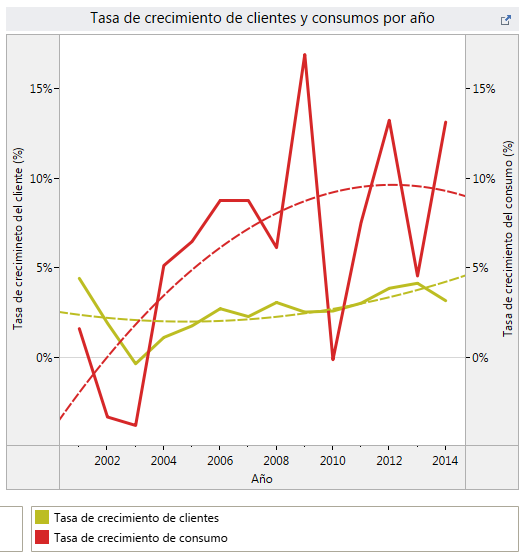
\includegraphics[width=\linewidth]{figuras/TasaDeCrecimientoVsConsumoDeEnergia2}
	\caption{Tasa de crecimiento vs Consumo de energ�a}
	\label{fig:TasaDeCrecimientoVsConsumoDeEnergia2}
\end{figure}}

En este gr�fico, titulado ``Proyecci�n de clientes y consumo para los pr�ximos 5 a�os`` se realiza una comparaci�n entre los clientes y el consumo de energ�a el�ctrica, similar que el gr�fico anterior, pero con la diferencia de que en este gr�fico se muestra la informaci�n con una unidad de medida diferente. A la izquierda tenemos el valor ``Cantidad de clientes`` y a la derecha el ``consumo`` en GWh.


\textsc{\begin{figure}[H]
	\centering
	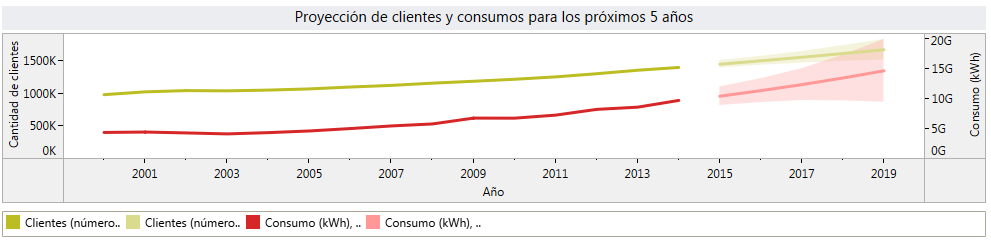
\includegraphics[width=\linewidth]{figuras/ProyeccionDeClientesYConsumosParaLosProximos5Anos}
	\caption{Proyecci�n de clientes y consumos para los pr�ximos 5 a�os}
	\label{fig:ProyeccionDeClientesYConsumosParaLosProximos5Anos}
\end{figure}}